\section{Decentralized search for \\ shortest path approximation}
\label{searching}

%\begin{figure*}[ht]
    %\centering
    %\subfigure[Decentralized search]{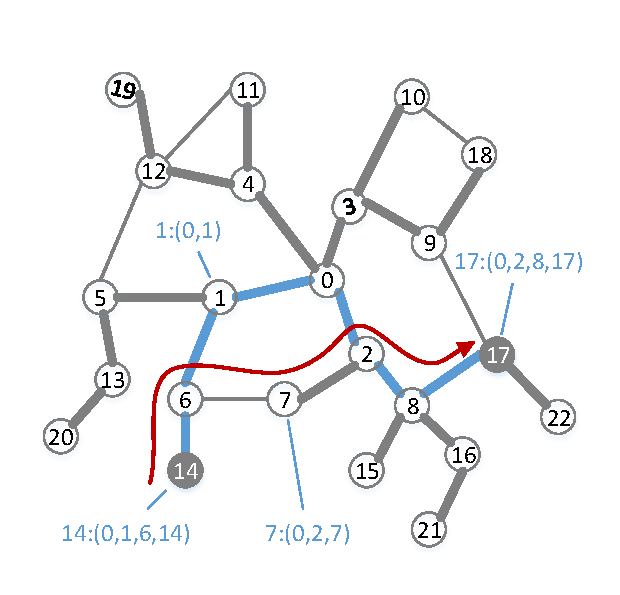
\epsfig{file=./figures/new_illustrate/ds_common.pdf,width=0.32\textwidth}\label{fig:DS:common}}
    %\subfigure[Bi-directional decentralized search]{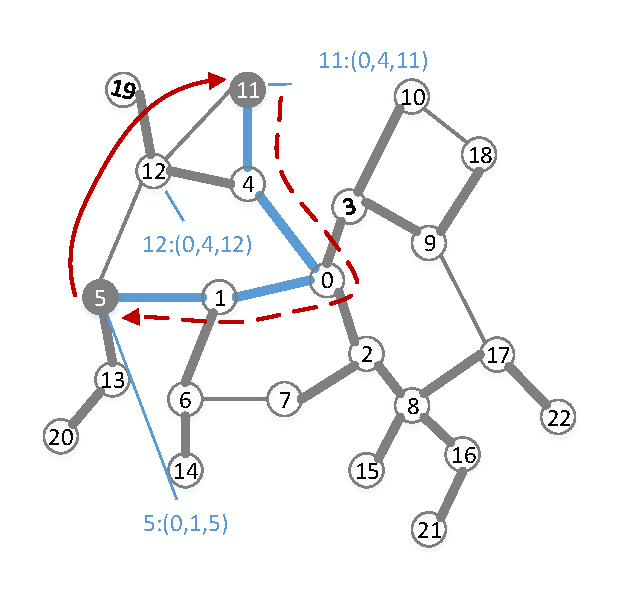
\epsfig{file=./figures/new_illustrate/ds_bidirectional.pdf,width=0.32\textwidth}\label{fig:DS:bidirectional}}
    %\subfigure[Tie breaking strategy]{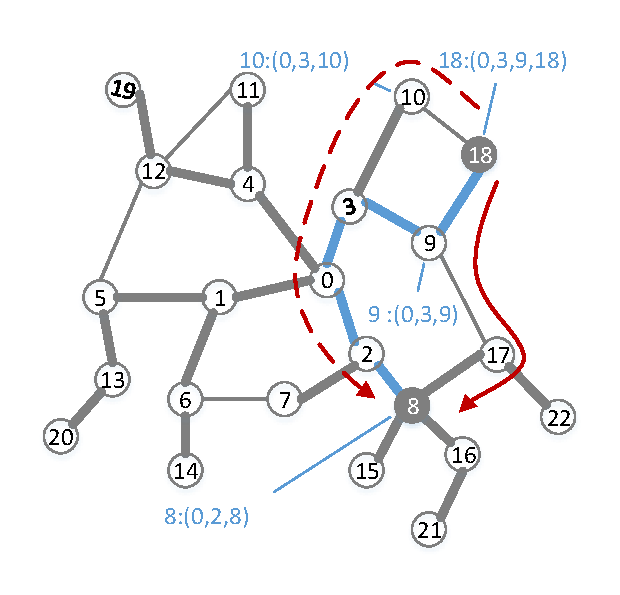
\epsfig{file=./figures/new_illustrate/ds_tie.pdf,width=0.32\textwidth}\label{fig:DS:tie}}
    %\caption{Examples of decentralized searches on indexed graphs. Bold lines denote the indexed edges. Curved lines denote paths being found, with arrows showing the directions. Dark vertices denote source and target vertices. Labels of vertices are shown in the $vertex:label$ format.}
%\end{figure*}

\begin{figure*}[ht]
		\vspace{-0.7cm}
    \centering
    \subfigure[Decentralized search 							 \label{fig:DS:common}]{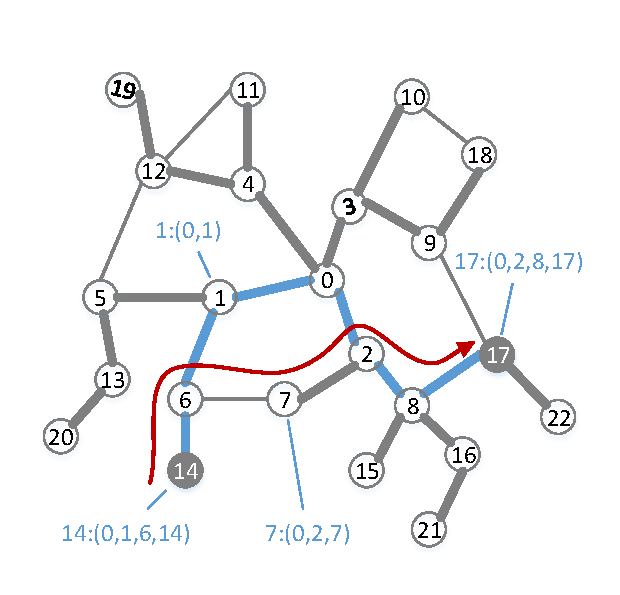
\includegraphics[width=0.32\textwidth]{figures/new_illustrate/ds_common.pdf}}
    \subfigure[Bi-directional decentralized search \label{fig:DS:bidirectional}]{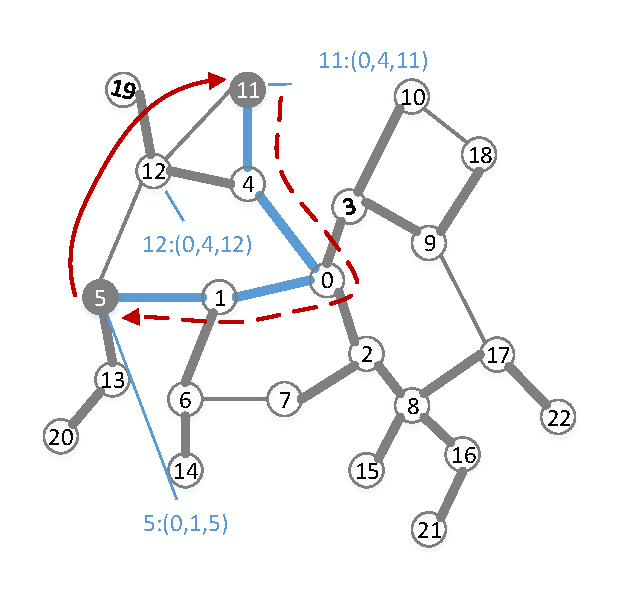
\includegraphics[width=0.32\textwidth]{figures/new_illustrate/ds_bidirectional.pdf}}
    \subfigure[Tie breaking strategy 							 \label{fig:DS:tie}]{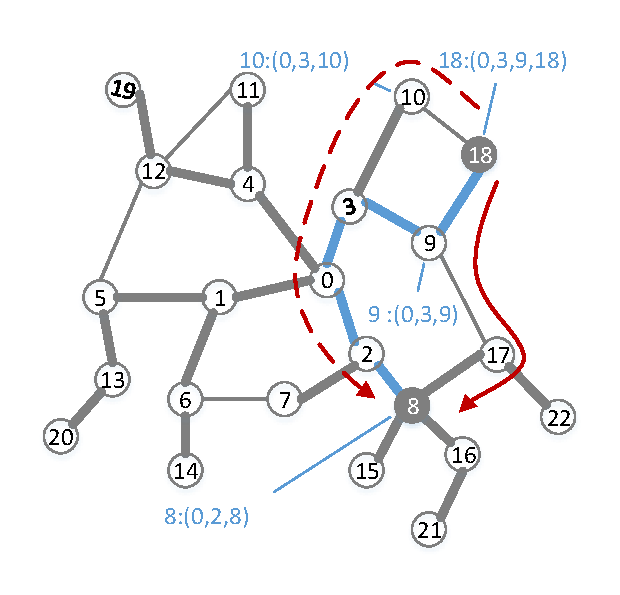
\includegraphics[width=0.32\textwidth]{figures/new_illustrate/ds_tie.pdf}}
    \caption{Examples of decentralized searches on indexed graphs. Bold lines denote the indexed edges. Curved lines denote paths being found, with arrows showing the directions. Dark vertices denote source and target vertices. Labels of vertices are shown in the $vertex:label$ format.}
\end{figure*}

We propose to solve the point-to-point shortest path approximation problem using decentralized search with landmark-based indexes. This section explains how to apply decentralized search on indexed graphs. Several aspects of the search, such as termination condition, bidirectional search and tie breaking strategy, are discussed.

\subsection{Index guided decentralized search}

To answer a shortest path query, decentralized search iteratively collects local distance information and visits the vertex with the least approximated distance to the target. More specifically, for a given pair of source $s$ and target vertex $t$ on an indexed graph, the search first sets the source vertex as the vertex to visit in the first step, and appends it to the approximated path $\tilde{p}(s,t)$. At each step, suppose that the search is visiting vertex $u$, it traverses all the neighbor vertices of $u$. For each neighbor vertex $v_i$, the metric $d_{LCA}(v_i,t)$ is calculated. Then the search sets the neighbor vertex with the smallest $d_{LCA}(v_i,t)$ as the vertex to visit in the next step, and appends $v_i$ to $\tilde{p}(s,t)$.

When the search reaches the target vertex, the search process naturally stops. However, this is not the ideal termination condition. We observe that, as shortest paths have optimal substructure, i.e., the path between any two vertices along a shortest path is also the shortest path of them, the search procedure can stop once it reaches an arbitrary vertex $u$, such that $u \in L(t)$ ($u$ is in the label of $t$. %meaning that a shortest path from $u$ to $t$ has been found). 
Evidently, decentralized search cannot find a shorter path than $p_L(u,t)$. The detailed algorithm of decentralized search is shown in Algorithm~\ref{alg:dec}.

\begin{algorithm}
    \caption{Decentralized search}
		\label{alg:dec}
    \begin{algorithmic}
        \Function{DecentralizedSearch}{$s$, $t$}
						\State $\tilde{p}(s,t) \gets \emptyset$
						\State $u \gets s$
						\State append $u$ to $\tilde{p}(s,t)$
						\While{$u \notin L(t)$}
								\State $d_{min} \gets \infty$
								\State $w \gets u$
								\For{each $v_i$ adjacent to $u$}
										\If{$d_{LCA}(v_i,t) < d_{min}$}
												\State $d_{min} \gets d_{LCA}(v_i,t)$
												\State $w \gets v_i$
										\EndIf
								\EndFor
								\State $u \gets w$
								\State append $u$ to $\tilde{p}(s,t)$
						\EndWhile
						\State $p_{remain} \gets p_L{u,t}$ excluding $u$
						\State append $p_{remain}$ to $\tilde{p}(s,t)$
						\State \Return $\tilde{p}(s,t)$
        \EndFunction
    \end{algorithmic}
\end{algorithm}

Observe that in this algorithm, by examining neighbor vertices, the search is able to explore a subset of the edges that are not indexed, to increase both accuracy and diversity of the path being found. For example, in Fig.~\ref{fig:DS:common}, observe that for the path from vertex $14$ to vertex $17$, decentralized search finds an edge $(6, 7)$ as vertex $7$ has a LCA distance of $3$, which is shorter than the LCA distance $5$ from vertex $1$ to $17$.

Regarding the termination condition, we have the following theorem:

\begin{theorem}
\label{theorem:max_step}
If the target vertex is reachable from the source, the decentralized search terminates in at most $2{\sigma}_{max}$ steps, where ${\sigma}_{max}$ is the diameter of the graph.
\end{theorem}
\begin{proof}[Proof Sketch]
For an arbitrary source vertex $s$ and a reachable target vertex $t$, the following bound holds:
\[
    d_{LCA}(s,t) = d_G(s,LCA(s,t)) + d_G(LCA(s,t),t) \leq 2{\sigma}_{max}
\]

Next, observe that at each step, decentralized search is visiting vertex $u$ and $u \neq t$. Assume the tightest upper bound in Equation (\ref{equ:upper}) is achieved on the shortest path tree $SPT_l$ rooted at landmark $l$. Let $v$ be the neighbor vertex of $u$ on the path $p_{LCA_l}(u,t)$. Since $SPT_l$ has no cycles, $p_{LCA_l}(v,t) \in p_{LCA_l}(u,t)$. Therefore the following equation holds:
\[
		d_{LCA}(v,t) = |p_{LCA_l}(v,t)| = |p_{LCA_l}(u,t)| - 1 = d_{LCA}(u,t) - 1
\]
Since decentralized search always picks the neighbor with shortest LCA distance to the target, the LCA distance to the target at each step decreases at least by $1$. Therefore, the decentralized search terminates in at most $2{\sigma}_{max}$ steps.
\end{proof}

The time complexity of the decentralized search procedure depends on the maximum degree and the diameter of the graph. As decentralized search takes at most $2{\sigma}_{max}$ steps to finish according to Theorem~\ref{theorem:max_step}, for each step, the search checks at most ${\delta}_{max}$ neighbor vertices, where ${\delta}_{max}$ is the maximum vertex degree of the graph. For each neighbor, $k$ LCA computations are required, and the time complexity for each LCA computation is $O(h)$\footnote{$O(h)$ is for simple online algorithm, off-line algorithms can achieve time complexity of $O(1)$~\cite{bender2000lca}.}, where $h$ is the height of the indexed shortest path tree and $h \leq {\sigma}_{max}$. Therefore, the worst case time complexity of decentralized search is $O(k{{\sigma}_{max}}^2{\delta}_{max})$. 
%Based on our experiments on real-world graphs, decentralized search can finish in much fewer steps and check much fewer vertices at each step. Therefore, decentralized search can finish much faster in most cases.

The space complexity for decentralized search contains two parts, space complexity for offline indexing, and space complexity for online query. The space required for offline indexing is $O(k{\sigma}_{max}n)$, where $n$ is the number of vertices. For each query, $O(k{\sigma}_{max})$ space is required to store the labels of target vertex and the vertex that is being examined. Therefore, $O(2{\sigma}_{max})$ space is required to store the approximated path. Combining them together, the online search space complexity of decentralized search is $O(k{\sigma}_{max})$.

\subsection{Bi-directional search}

In this section, we show how to apply the idea of bidirectional search to decentralized search. In bidirectional decentralized search, the backward search starts at the target vertex and is driven by the goal to reach the source vertex. The forward search and backward search may explore different search spaces due to this difference. By exploring a different search space, the backward search may find a shorter approximated path. This, however, is quite different from the application of bidirectional search in BFS or A* search where the main focus is to reduce search space.

An example of directional decentralized search is shown in Fig.~\ref{fig:DS:bidirectional}. Let $11$ be the source and $5$ be the target. The backward search can find a shorter path $p_{bwd} = (5, 12, 11)$ than the path $p_{fwd} = (11, 4, 0, 1, 5)$ by the forward search. The backward search finds a shorter path by exploring edge $(5, 12)$. However, this edge is invisible to the forward search because when the search traverses vertex $4$, it prioritizes $0$ than $12$ due to the former one has a lower LDA distance to the target vertex $5$.

It is not guaranteed that the forward search and the backward search will eventually meet at any intermediate vertex. As shown in our previous example, $p_{fwd} \cap p_{bwd} = (11, 5)$. Actually, in decentralized search, the forward search and backward search are mostly two independent searches, where the only interaction of them is when the search results are combined, where the shorter paths are returned. 

\subsection{Tie breaking strategy}

Ties happen frequently in decentralized search, especially when the number of landmarks is small. In the decentralized search, a tie means multiple neighbor vertices have same LCA distance to the target in a step. 
%The reason that a tie happens is that there is not sufficient information in indexes that can separate neighbor vertices for a query. 
For example, in Fig.~\ref{fig:DS:tie}, consider a search from $18$ to $8$. When traversing neighbors of vertex $18$, both vertex $10$ and $9$ have the same LCA distances to target vertex $8$, but their actual distances to vertex $8$ are different, due to that the shortcut edge $(9, 17)$ is currently invisible to the decentralized search.

The search space of the decentralized search can be increased by expanding the search onto each tied vertex. This increases both the performance, i.e., chances to find a shorter path and the number of paths being found, and the cost of the search. By controlling the search space this way, decentralized search is able to achieve different levels of accuracy.

Two extreme ways to deal with ties are either only visiting one vertex, or visiting all vertices in the next step. The former one incurs the least search cost, and has the least possibility to find a shorter path. We refer to it as single branch decentralized search. The latter one requires most effort and can lead to the shortest path the decentralized search could possibly find. We refer to it as full branch decentralized search.

\subsection{Extension on directed graphs}
To treat directed graphs, for each landmark, the label of a vertex $u$ need to store both the path from the landmark to the vertex, denoted as $p_{l \rightarrow u}$, and the path from the vertex to the landmark, denoted as $p_{u \rightarrow l}$. When the search is visiting vertex $u$, only out-edges of $u$ need to be traversed. To calculate LCA distance from $u$ to the target vertex $t$, $p_{l \rightarrow u}$ is used for $u$ and $p_{t \rightarrow l}$ is used.
